\documentclass[11pt]{article}

\usepackage[a4paper,margin=1in]{geometry}
\usepackage[utf8]{inputenc}
\usepackage[T1]{fontenc}
\usepackage{lmodern}
\usepackage{microtype}

\usepackage{amsmath,amssymb,amsthm,mathtools}
\usepackage{booktabs}
\usepackage{array}
\usepackage{enumitem}
\usepackage{xcolor}
\usepackage{listings}
\usepackage{tikz}
\usetikzlibrary{arrows.meta}
\usepackage[hidelinks]{hyperref}
\usepackage{cleveref}

% --- code listings -----------------------------------------------------------
\definecolor{codegray}{gray}{0.96}
\definecolor{codecmnt}{rgb}{0.25,0.50,0.25}
\definecolor{codekw}{rgb}{0.10,0.10,0.55}
\definecolor{codestr}{rgb}{0.55,0.10,0.10}

\lstset{
  basicstyle=\ttfamily\footnotesize,
  backgroundcolor=\color{codegray},
  keywordstyle=\color{codekw}\bfseries,
  commentstyle=\color{codecmnt}\itshape,
  stringstyle=\color{codestr},
  numbers=left, numberstyle=\tiny\color{gray},
  stepnumber=1, numbersep=6pt,
  frame=single, framerule=0pt,
  breaklines=true, breakatwhitespace=true,
  showstringspaces=false,
  captionpos=b,
  language=C,
  morekeywords={int64_t,size_t,bool,struct,MPI_Init,MPI_Comm_rank,MPI_Comm_size,
                MPI_Allreduce,MPI_Cart_create,MPI_Cart_get,MPI_Finalize}
}

% --- theorem environments ----------------------------------------------------
\newtheorem{theorem}{Theorem}
\newtheorem{proposition}[theorem]{Proposition}
\newtheorem{lemma}[theorem]{Lemma}
\theoremstyle{definition}
\newtheorem{definition}[theorem]{Definition}
\newtheorem{remark}[theorem]{Remark}

% --- macros ------------------------------------------------------------------
\newcommand{\R}{\mathbb{R}}
\newcommand{\Z}{\mathbb{Z}}
\newcommand{\N}{\mathbb{N}}
\newcommand{\bx}{\mathbf{x}}
\newcommand{\norm}[1]{\left\lVert #1 \right\rVert}
\newcommand{\abs}[1]{\left\lvert #1 \right\rvert}
\newcommand{\Linf}{L^{\infty}}
\newcommand{\bigO}{\mathcal{O}}
\DeclareMathOperator{\diag}{diag}
\DeclareMathOperator{\spr}{\rho}

\title{A Parallel Geometric Multigrid Solver for the 3D Poisson Equation:\\
       Algorithm, Implementation, and Extension Guide}
\author{Documentation for the \texttt{Multigrid} code base\\
        \small (HPC for Mathematical Modelling, PhD course notes)}
\date{\today}

\begin{document}
\maketitle

\begin{abstract}
This document describes the analytic problem, discretisation, and
parallel multigrid algorithm implemented in the accompanying code base.
The implementation solves the three-dimensional Poisson equation on
the unit cube with homogeneous Dirichlet boundary conditions, using a
node-based seven-point finite-difference Laplacian, a red-black
Gauss--Seidel smoother with successive over-relaxation, and a geometric
V-cycle multigrid acceleration on a halved-grid hierarchy.  The code is
parallelised with MPI through a Cartesian process topology and ghost-zone
communication.  We give a self-contained presentation aimed at a PhD-level
audience in high-performance computing for mathematical modelling, then
document the user-selectable parameters and explain how to extend the
solver to other source terms and to non-homogeneous Dirichlet, Neumann,
and Robin boundary conditions.  Standard references are
\cite{briggs2000multigrid,trottenberg2001multigrid,hackbusch1985multi,
saad2003iterative,leveque2007finite}.
\end{abstract}

\tableofcontents
\bigskip

% =============================================================================
\section{Introduction}
% =============================================================================

The Poisson equation $-\Delta u = f$ is the canonical elliptic boundary-value
problem and the standard test bed for elliptic solvers.  Its symmetric,
positive-definite, sparse algebraic structure --- combined with the fact
that classical relaxation methods (Jacobi, Gauss--Seidel, SOR) are very
effective at damping high-frequency error components but very poor at
damping low-frequency components --- makes it the textbook target for
\emph{multigrid} methods, which combine a smoother on each level of a
grid hierarchy with coarse-grid correction
\cite{brandt1977multilevel,fedorenko1964relaxation,
hackbusch1985multi,trottenberg2001multigrid}.  Multigrid is the
asymptotically optimal solver for the discrete Poisson problem: it
reduces the algebraic error by a fixed factor in
$\bigO(N)$ work, where $N$ is the number of unknowns
\cite[Ch.~5]{briggs2000multigrid}.

This document describes a \emph{parallel} geometric multigrid implementation
written in C with MPI.  It is organised as follows:
\Cref{sec:problem} states the continuous problem;
\Cref{sec:discretisation} the finite-difference discretisation;
\Cref{sec:relaxation} reviews the relaxation methods that serve as
smoothers; \Cref{sec:multigrid} develops the geometric multigrid theory
needed to follow the implementation; \Cref{sec:implementation} is a
guided tour of the code; \Cref{sec:parameters} documents the user
parameters with practical tuning guidance; and \Cref{sec:extension}
explains how to extend the code to other right-hand sides and boundary
conditions.

% =============================================================================
\section{The continuous problem}\label{sec:problem}
% =============================================================================

Let $\Omega = (0,1)^3 \subset \R^3$.  We seek $u\colon\overline{\Omega}\to\R$
satisfying
\begin{equation}\label{eq:poisson}
  \Delta u(\bx) = f(\bx)\quad \text{in } \Omega,\qquad
  u(\bx) = 0 \quad \text{on } \partial\Omega,
\end{equation}
where $\Delta = \partial_{xx} + \partial_{yy} + \partial_{zz}$ and $f \in
L^2(\Omega)$.  The associated weak formulation is: find $u\in H^1_0(\Omega)$ such
that
\begin{equation}\label{eq:weak}
  \int_\Omega \nabla u \cdot \nabla v \,d\bx
  = -\int_\Omega f v \, d\bx
  \qquad \forall v \in H^1_0(\Omega).
\end{equation}
By the Lax--Milgram lemma this problem has a unique solution in $H^1_0(\Omega)$
\cite[Ch.~6]{evans2010pde}, and on a convex domain such as the unit cube
the solution lies in $H^2(\Omega)\cap H^1_0(\Omega)$ with the elliptic-regularity
estimate $\norm{u}_{H^2}\le C \norm{f}_{L^2}$.

The driver currently uses the manufactured smooth solution
\begin{equation}\label{eq:manufactured}
  u_\star(\bx) = \sin(\pi x)\sin(\pi y)\sin(\pi z),\qquad
  f_\star(\bx) = -3\pi^2 \sin(\pi x)\sin(\pi y)\sin(\pi z),
\end{equation}
so that $\Delta u_\star = f_\star$ and $u_\star \equiv 0$ on $\partial\Omega$.
This choice provides a closed-form reference for measuring the
discretisation error.

\begin{remark}[Sign convention]
The implementation writes the equation as $\Delta u = f$ with $f =
-3\pi^2 \sin(\pi x)\sin(\pi y)\sin(\pi z)$, not the more common form
$-\Delta u = g$.  The two are equivalent under $g=-f$.  The
\emph{defect} computed by the code is
$d = \Delta_h u_h - f_h$, where $\Delta_h$ denotes the discrete
Laplacian; \emph{not} $f_h - \Delta_h u_h$.  This sign propagates
through the multigrid update --- in particular, the prolongation
operator subtracts (rather than adds) the coarse correction
(\Cref{sec:prolongation}).
\end{remark}

% =============================================================================
\section{Discretisation}\label{sec:discretisation}
% =============================================================================

\subsection{Node-based grid}
We discretise $\overline{\Omega}$ with a uniform tensor-product grid
\begin{equation*}
  \bx_{ijk} = (i\,h_x,\,j\,h_y,\,k\,h_z),\quad
  i=0,\dots,N_x-1,\ j=0,\dots,N_y-1,\ k=0,\dots,N_z-1,
\end{equation*}
where $N_x = n_x+1$, $N_y = n_y+1$, $N_z = n_z+1$ and $h_x = 1/n_x$,
$h_y = 1/n_y$, $h_z = 1/n_z$.  The user specifies the cell counts $n_x$,
$n_y$, $n_z$ in the input file; the corresponding number of
\emph{grid points} per axis is one larger.  The boundary nodes $i\in\{0,N_x-1\}$
(and similarly $j,k$) are Dirichlet nodes and are not unknowns of the
linear system.

\subsection{Seven-point Laplacian}
We approximate $\Delta u$ by the standard second-order central
difference
\begin{equation}\label{eq:laplacian-7pt}
  \Delta_h u_{ijk} \;\coloneqq\;
  \frac{u_{i+1,j,k}-2u_{ijk}+u_{i-1,j,k}}{h_x^2}
  +\frac{u_{i,j+1,k}-2u_{ijk}+u_{i,j-1,k}}{h_y^2}
  +\frac{u_{i,j,k+1}-2u_{ijk}+u_{i,j,k-1}}{h_z^2}.
\end{equation}
Taylor expansion around $\bx_{ijk}$ shows that, for $u\in C^4(\overline\Omega)$,
the truncation error satisfies
\begin{equation}\label{eq:truncation}
  \Delta_h u(\bx_{ijk}) - \Delta u(\bx_{ijk})
  = \tfrac{h_x^2}{12} \partial_x^4 u + \tfrac{h_y^2}{12}\partial_y^4 u
  + \tfrac{h_z^2}{12}\partial_z^4 u + \bigO(h^4),
\end{equation}
so the scheme is second-order consistent in $h\coloneqq\max(h_x,h_y,h_z)$
\cite[Ch.~2]{leveque2007finite}.  Combined with discrete-maximum-principle
stability, this yields second-order convergence in the $\ell^\infty$ norm,
$\norm{u_h - u}_{\ell^\infty(\Omega_h)} = \bigO(h^2)$
\cite[Ch.~2--3]{leveque2007finite}.

The discrete system $A_h u_h = f_h$ has a symmetric, negative-definite,
$M$-matrix structure with seven non-zeros per interior row and is
the standard model problem in the multigrid literature
\cite[\S2.1]{trottenberg2001multigrid}.

\subsection{Index convention and storage}
The code stores the unknowns in a flat array with the linear index
\begin{equation*}
  \mathrm{idx}(i,j,k) \;=\; i + (j + k\,N_y)\,N_x,
\end{equation*}
so that $i$ is the unit-stride (innermost) axis.  This is the
\texttt{gf\_indx\_3d} macro in \texttt{gf.h}.  Each rank holds a
contiguous tile of grid points plus a single layer of \emph{ghost} cells
on every face that is shared with another rank
(\Cref{fig:ghost}).  The ghost width is fixed at $g_s = 1$,
matching the seven-point stencil.

\subsection{Per-axis layout for cell-centred
  Neumann}\label{sec:cell-centred-layout}
The grid above is \emph{vertex-centred}: a grid point lies on each
physical-boundary face, which is the natural layout for Dirichlet BCs
($u$ is prescribed at the boundary node).  For Neumann BCs the
discrete compatibility $\sum f_h = 2\sum_{\partial\Omega} q/h$ does
not match the continuous compatibility $\int f = \int q$, a
factor-of-two artefact of the boundary node carrying full-cell
weight in the row sum.  We therefore use a different layout
\emph{per axis}, chosen by the BC pair on that axis.

\Cref{fig:axis-layouts} shows the four configurations in 1D
(the choice is independent on each axis, so the 3D layout is the
tensor product of three 1D layouts).  Filled circles are interior
cell or vertex \emph{values stored at that slot}; the square marker
is the Dirichlet vertex slot, whose value is fixed by
\texttt{apply\_bc\_3d} from the per-face callback; open circles are
Neumann ghost slots, whose value is set by the mirror formula.  The
domain boundary $x = a_a$ or $x = b_a$ is the vertical dashed line;
crucially, on cell-centred axes the boundary does \emph{not}
coincide with a stored slot -- it falls between the first interior
cell centre and its Neumann ghost.

\begin{figure}[ht]
\centering
\newcommand{\axisrow}[2]{%
  % #1 = label (top), #2 = drawing commands
  \begin{tikzpicture}[scale=0.95,>=stealth,line width=0.4pt]
    \node[anchor=west] at (-0.8,1.1) {\textbf{#1}};
    \draw[->,thick] (-1.1,0) -- (5.4,0) node[right] {$x$};
    #2
  \end{tikzpicture}}
% --- D--D (vertex-centred): N+1 vertices, both ends Dirichlet ---
\axisrow{D--D axis: $N_a{+}1$ vertex-centred slots
        ($i = 0, \dots, N_a$)}{%
  % domain boundaries
  \draw[dashed,thick,gray!70] (0,-1.1) -- (0,0.95);
  \draw[dashed,thick,gray!70] (4,-1.1) -- (4,0.95);
  \node[gray!60!black,font=\scriptsize] at (0,-1.0) {$x = a_a$};
  \node[gray!60!black,font=\scriptsize] at (4,-1.0) {$x = b_a$};
  % three interior vertices are filled circles, the two ends are
  % Dirichlet vertices drawn as filled squares (boundary coincides
  % with stored slot)
  \foreach \i in {1,2,3} {
    \filldraw (\i,0) circle (0.08);
    \node[below=4pt] at (\i,-0.1) {\scriptsize $i{=}\i$};}
  \draw[fill=black] (-0.08,-0.08) rectangle (0.08,0.08);
  \draw[fill=black] (4-0.08,-0.08) rectangle (4+0.08,0.08);
  \node[below=4pt] at (0,-0.1) {\scriptsize $i{=}0$};
  \node[below=4pt] at (4,-0.1) {\scriptsize $i{=}N_a$};
  \node[above=2pt] at (0,0.1) {\scriptsize $u_v$};
  \node[above=2pt] at (4,0.1) {\scriptsize $u_v$};
}

\vspace{1em}

% --- N--N (cell-centred): N+2 slots, two ghosts ---
\axisrow{N--N axis: $N_a{+}2$ cell-centred slots
        ($i = 0, \dots, N_a{+}1$, two ghosts)}{%
  \draw[dashed,thick,gray!70] (0,-1.1) -- (0,0.95);
  \draw[dashed,thick,gray!70] (4,-1.1) -- (4,0.95);
  \node[gray!60!black,font=\scriptsize] at (0,-1.0) {$x = a_a$};
  \node[gray!60!black,font=\scriptsize] at (4,-1.0) {$x = b_a$};
  % interior cell centres at h/2, 3h/2, 5h/2, 7h/2 (four cells for N=4)
  \foreach \pos/\lab in {0.5/1, 1.5/2, 2.5/3, 3.5/4} {
    \filldraw (\pos,0) circle (0.08);
    \node[below=4pt] at (\pos,-0.1) {\scriptsize $i{=}\lab$};}
  % Neumann ghost slots at -h/2 and (N+1/2)h
  \draw[fill=white,line width=0.6pt] (-0.5,0) circle (0.08);
  \draw[fill=white,line width=0.6pt] (4.5,0) circle (0.08);
  \node[below=4pt] at (-0.5,-0.1) {\scriptsize $i{=}0$};
  \node[below=4pt] at (4.5,-0.1) {\scriptsize $i{=}N_a{+}1$};
  \node[above=2pt] at (-0.5,0.1) {\scriptsize ghost};
  \node[above=2pt] at (4.5,0.1) {\scriptsize ghost};
}

\vspace{1em}

% --- D--N (hybrid): N+2 slots, D vertex at lower, N ghost at upper ---
\axisrow{D--N axis: $N_a{+}2$ slots, D vertex on lower face}{%
  \draw[dashed,thick,gray!70] (0,-0.75) -- (0,0.75);
  \draw[dashed,thick,gray!70] (4,-0.75) -- (4,0.75);
  \node[gray!60!black,font=\scriptsize] at (0,-1.0) {$x = a_a$};
  \node[gray!60!black,font=\scriptsize] at (4,-1.0) {$x = b_a$};
  % Dirichlet vertex at x = a (i=0)
  \draw[fill=black] (-0.08,-0.08) rectangle (0.08,0.08);
  \node[below=4pt] at (-.2,-0.1) {\scriptsize $i{=}0$};
  \node[above=2pt] at (0,0.1) {\scriptsize $u_v$};
  % interior cell centres at h/2, 3h/2, 5h/2, 7h/2 (i=1..4)
  \foreach \pos/\lab in {0.5/1, 1.5/2, 2.5/3, 3.5/4} {
    \filldraw (\pos,0) circle (0.08);
    \node[below=4pt] at (\pos,-0.1) {\scriptsize $i{=}\lab$};}
  % Neumann ghost at (N+1/2)h
  \draw[fill=white,line width=0.6pt] (4.5,0) circle (0.08);
  \node[below=4pt] at (4.6,-0.1) {\scriptsize $i{=}N_a{+}1$};
  \node[above=2pt] at (4.5,0.1) {\scriptsize ghost};
  % half-step indicator
  \draw[<->,thin,gray] (0,0.65) -- (0.5,0.65);
  \node[gray!60!black,font=\scriptsize] at (0.25,0.8) {$h_a/2$};
}

\vspace{1em}

% --- N--D (hybrid): N+2 slots, N ghost at lower, D vertex at upper ---
\axisrow{N--D axis: $N_a{+}2$ slots, D vertex on upper face}{%
  \draw[dashed,thick,gray!70] (0,-.75) -- (0,0.75);
  \draw[dashed,thick,gray!70] (4,-.75) -- (4,0.75);
  \node[gray!60!black,font=\scriptsize] at (0,-1.0) {$x = a_a$};
  \node[gray!60!black,font=\scriptsize] at (4,-1.0) {$x = b_a$};
  % Neumann ghost at -h/2 (i=0)
  \draw[fill=white,line width=0.6pt] (-0.5,0) circle (0.08);
  \node[below=4pt] at (-0.5,-0.1) {\scriptsize $i{=}0$};
  \node[above=2pt] at (-0.5,0.1) {\scriptsize ghost};
  % interior cell centres at h/2, 3h/2, 5h/2, 7h/2 (i=1..3);
  % the i=4 label is anchored east (text extends LEFT from x=3.5)
  % so it sits clear of the wider i=Na+1 label at x=4.
  \foreach \pos/\lab in {0.5/1, 1.5/2, 2.5/3} {
    \filldraw (\pos,0) circle (0.08);
    \node[below=4pt] at (\pos,-0.1) {\scriptsize $i{=}\lab$};}
  \filldraw (3.5,0) circle (0.08);
  \node[anchor=north east,font=\scriptsize] at (3.45,-0.18) {$i{=}4$};
  % Dirichlet vertex at x = b (i=N+1); label anchored west (text
  % extends RIGHT from x=4) so it does not collide with i=4.
  \draw[fill=black] (4-0.08,-0.08) rectangle (4+0.08,0.08);
  \node[anchor=north west,font=\scriptsize] at (4.05,-0.18) {$i{=}N_a{+}1$};
  \node[above=2pt] at (4,0.1) {\scriptsize $u_v$};
  % half-step indicator
  \draw[<->,thin,gray] (3.5,0.70) -- (4,0.70);
  \node[gray!60!black,font=\scriptsize] at (3.75,0.85) {$h_a/2$};
}
\caption{Per-axis grid layouts ($N_a = 4$ cells shown).  Filled
circles: interior cell centres.  Filled squares: Dirichlet vertex
slots (value set by \texttt{apply\_bc\_3d} at the boundary
coordinate).  Open circles: Neumann ghost slots (value set by the
mirror formula $u_{\text{ghost}} = u_{\text{int}} + h_a\,q$).
Dashed lines mark the physical-boundary coordinates $x = a_a$ and
$x = b_a$.  The half-step $h_a/2$ between a Dirichlet vertex and
the first interior cell centre is the defining feature of hybrid
axes.}
\label{fig:axis-layouts}
\end{figure}

The four cases differ in stored-slot count and spacing:
\begin{itemize}
  \item \textbf{D--D axis} (both ends Dirichlet): $N_a + 1$
    vertex-centred slots at $x = a_a + i h_a$, $i = 0, \dots, N_a$.
    The two end slots hold Dirichlet vertex values; uniform spacing
    $h_a$ throughout.
  \item \textbf{N--N axis} (both ends Neumann): $N_a + 2$ slots,
    lowest at $a_a - h_a/2$, highest at $b_a + h_a/2$, uniform
    spacing $h_a$.  The two extreme slots are \emph{ghost cells};
    \texttt{apply\_bc\_3d} writes them via the centred-difference
    Neumann mirror
    $u_{\text{ghost}} = u_{\text{int}} + h_a\,q$, where
    $q = \partial u/\partial n$ at the boundary plane (midway
    between the ghost and the first interior cell centre).
    Compatibility becomes
    $\sum f_h = \sum_{\partial\Omega} q/h$, matching the
    continuous condition under midpoint quadrature.
  \item \textbf{D--N or N--D axis} (hybrid): $N_a + 2$ slots; one
    end is a Dirichlet vertex placed exactly at the boundary
    coordinate, the other is a Neumann ghost half a cell outside.
    A single half-step $h_a/2$ separates the Dirichlet vertex from
    the first interior cell centre on that axis; all other
    spacings are $h_a$.  The cell adjacent to the Dirichlet vertex
    uses a non-uniform 4-point one-sided second-derivative on that
    axis (\Cref{sec:smoother-impl}); other cells use the standard
    centred-difference stencil.
\end{itemize}

The layout is encoded by per-face Neumann flags carried on
\texttt{struct domain3d\_st}; the choice of layout is uniform across
every multigrid level (\Cref{sec:hierarchy}) and is a property of
the problem, not of the grid resolution.  Pure D--D problems are
unaffected by these changes.

\paragraph{Endpoint slots and the $L^\infty$ metric.}
On any axis with a Neumann face, the cell-centred coordinate that
the formula $x_i = x_0^{\text{(shifted)}} + i h_a$ produces at the
endpoint slots does not coincide with the value
\texttt{apply\_bc\_3d} stored there: a pure-Neumann ghost holds the
mirror value (no physical interpretation at its formula coordinate),
and a hybrid Dirichlet vertex holds the boundary value at the face
coordinate (which is $h_a/2$ from its formula coordinate).
\texttt{problem\_compute\_max\_error} accordingly skips both
endpoint slots on Neumann-bearing axes; pure D--D axes keep both
endpoints (the formula coordinate coincides with the boundary).
The output writer's \texttt{owned\_bounds\_3d} helper applies the
same rule, so the assembled global field rendered by
\texttt{scripts/make\_xdmf.py} matches the values that the metric
sees.

% =============================================================================
\section{Stationary relaxation methods}\label{sec:relaxation}
% =============================================================================

Before turning to multigrid, we recall the building blocks the smoother
is composed of.  Let $A_h u_h = f_h$ be the discrete system from
\eqref{eq:laplacian-7pt}, with $A_h = D - L - U$ where $D$ is the diagonal
and $L$, $U$ are the strict lower/upper-triangular parts.

\subsection{Jacobi, Gauss--Seidel, SOR}
The \emph{Gauss--Seidel} (GS) iteration is
$u^{(m+1)} = (D-L)^{-1}(U u^{(m)} + f_h)$, i.e. each unknown is updated
in turn using the most recent values of its neighbours.  The
\emph{successive over-relaxation} (SOR) method introduces a relaxation
parameter $\omega>0$:
\begin{equation}\label{eq:sor}
  u^{(m+1)}_{ijk}
  = (1-\omega)\,u^{(m)}_{ijk} + \omega\,\widetilde u_{ijk},\qquad
  \widetilde u_{ijk} = \frac{f_{ijk} - \sum_{(p,q,r)\ne(0,0,0)} a_{ijk;pqr}
  u_{i+p,j+q,k+r}}{a_{ijk;000}},
\end{equation}
where $\widetilde u_{ijk}$ is the standard GS update.  For SPD matrices,
SOR converges if and only if $0<\omega<2$ \cite[Thm.~10.1.2]{golub2013matrix};
$\omega=1$ recovers Gauss--Seidel.

For the constant-coefficient five-point Laplacian on an $n\times n$
square grid, Young's classical analysis yields the optimal parameter
\begin{equation}\label{eq:omega-opt}
  \omega_{\mathrm{opt}} = \frac{2}{1 + \sin(\pi h)} \;\approx\; 2 - 2\pi h
  \quad \text{as } h\to 0,
\end{equation}
with asymptotic spectral radius $\spr_{\mathrm{opt}} = \omega_{\mathrm{opt}}
- 1 \approx 1 - 2\pi h$, i.e.\ a convergence rate of $\bigO(h)$ rather than
the $\bigO(h^2)$ rate of plain Gauss--Seidel
\cite[Ch.~5]{young1971iterative},
\cite[\S4.2.2]{saad2003iterative},
\cite[Ch.~3]{varga2009matrix}.  In three dimensions the analogous
formula has the same leading behaviour
\cite[\S2.5]{trottenberg2001multigrid}.

\subsection{Smoothing property of relaxation}\label{sec:smoothing-property}
The reason classical relaxation appears in multigrid is not its global
convergence rate but its \emph{smoothing} property: the high-frequency
components of the error are damped quickly even when the low-frequency
components are not.  For the discrete Laplacian, expand the error
$e^{(m)} = u_h - u^{(m)}$ in the Fourier basis.  The Jacobi/GS/SOR
amplification factor depends on the wavenumber $\theta$.  For
weighted Jacobi and Gauss--Seidel applied to the model problem, the
smoothing factor (the worst amplification factor over high-frequency
modes $\theta\in[\pi/2,\pi]$) is bounded away from 1 uniformly in $h$
\cite[\S2.1]{trottenberg2001multigrid},
\cite[\S3.2]{briggs2000multigrid}.  This is the property that makes
multigrid work.

\subsection{Red-black ordering}\label{sec:redblack}
The Gauss--Seidel iteration is sequential as written, because updating
$u_{ijk}$ requires the already-updated $u_{i-1,j,k}$, $u_{i,j-1,k}$,
$u_{i,j,k-1}$.  For the seven-point stencil this dependency disappears
under a \emph{red-black} (or \emph{checkerboard}) ordering: we colour
each grid point with parity $c(i,j,k)= (i+j+k)\bmod 2$, then update
all red points first (every red neighbour stencil consists only of
black points, which are not being updated), exchange ghosts, and
finally update all black points.  The resulting iteration is a
genuine Gauss--Seidel iteration with respect to the red-black
permutation, but each half-sweep is fully parallel.  For the
five-point Laplacian, red-black GS has smoothing factor exactly $1/4$
in two dimensions, independent of $h$
\cite[\S3.2]{trottenberg2001multigrid}; the three-dimensional
seven-point case has the same qualitative behaviour.

% =============================================================================
\section{Geometric multigrid}\label{sec:multigrid}
% =============================================================================

This section condenses the parts of the multigrid story that are needed to
read the code; the canonical references are
\cite{briggs2000multigrid,trottenberg2001multigrid,hackbusch1985multi}.

\subsection{Two-grid idea}
Suppose we have a fine grid $\Omega_h$ with operator $A_h$ and a coarse
grid $\Omega_H$ (with $H=2h$) with operator $A_H$, plus
\begin{itemize}[nosep]
  \item a \emph{restriction} $R_h^H : \Omega_h \to \Omega_H$, transferring
    fine-grid functions to the coarse grid;
  \item a \emph{prolongation} $P_H^h : \Omega_H \to \Omega_h$, transferring
    coarse-grid functions to the fine grid.
\end{itemize}
After a few sweeps of relaxation on $A_h u_h = f_h$, the error
$e = u_h^\star - u_h$ is smooth and therefore well representable on
$\Omega_H$.  The two-grid cycle reads:
\begin{enumerate}[leftmargin=*,nosep]
  \item Pre-smooth: $u_h \leftarrow S_h^{\nu_1}(u_h, f_h)$.
  \item Compute the defect $d_h = A_h u_h - f_h$ (note the sign convention
    of \Cref{sec:problem}).
  \item Restrict: $d_H = R_h^H d_h$.
  \item Solve the coarse defect equation
    $A_H e_H = d_H$ (exactly or approximately).
  \item Prolong and \emph{subtract} the correction:
    $u_h \leftarrow u_h - P_H^h e_H$.
  \item Post-smooth: $u_h \leftarrow S_h^{\nu_2}(u_h, f_h)$.
\end{enumerate}

\subsection{V-cycle and W-cycle}
Recursively replacing the exact solve in step 4 with $\gamma$ applications
of the same cycle defines the \emph{multigrid cycle of index $\gamma$}:
$\gamma=1$ is a V-cycle, $\gamma=2$ is a W-cycle
\cite[Fig.~3.1]{trottenberg2001multigrid}.  In the present code the
parameter \texttt{subcycles} controls $\gamma$ at every level (see
\Cref{sec:vcycle-impl}).

\begin{theorem}[Multigrid optimality, informal]\label{thm:mg}
For the discrete Poisson problem with full-weighting restriction,
linear interpolation, and a sufficient number of relaxation sweeps,
the V-cycle reduces the error by a factor that is bounded away from 1
\emph{uniformly in $h$}.  The cost of one V-cycle is $\bigO(N)$ where
$N$ is the number of fine-grid unknowns, so the total cost of obtaining
a discretisation-accurate solution is $\bigO(N)$.
\end{theorem}

A precise statement and proof under the appropriate regularity and
approximation hypotheses is given in
\cite[Ch.~6]{hackbusch1985multi} and \cite[Ch.~7]{trottenberg2001multigrid}.

\subsection{Transfer operators}\label{sec:transfer}
The code carries \emph{two} pairs of transfer operators and picks one
at every level based on the per-axis layout
(\Cref{sec:cell-centred-layout}):
\begin{itemize}
\item If every axis is \emph{purely Dirichlet} (D--D on all three),
  the level uses the historical vertex-centred operators
  \texttt{inject\_var\_3d} + \texttt{restrict\_var\_3d} (full-weighting
  restriction) and \texttt{prolong\_var\_3d} (trilinear interpolation),
  documented in
  \Cref{sec:transfer-dd}.
\item If \emph{any} axis carries at least one Neumann face (the
  remaining seven of the eight 3-axis combinations: NN-DD-DD,
  hybrid-DD-DD, NN-NN-DD, hybrid-hybrid-DD, NN-NN-NN, etc.),
  the level uses the cell-centred operators
  \texttt{restrict\_var\_cc\_3d} (box-average restriction) and
  \texttt{prolong\_var\_cc\_3d} (cc trilinear interpolation with a
  position-aware override at hybrid Dirichlet vertices), documented
  in \Cref{sec:transfer-cc}.
\end{itemize}
The choice is made once at hierarchy-construction time and persists
across every level (the layout is invariant under coarsening; see
\Cref{sec:hierarchy}).  Both pairs are second-order accurate; the
cc pair is what enables a uniform stencil across every Neumann face
without the half-cell offset and the discrete compatibility mismatch
that the vertex-centred pair would introduce.

\subsubsection{Vertex-centred operators (D--D axes)}\label{sec:transfer-dd}
On every axis the coarse-grid index $I$ maps to the fine-grid index
$2I$; the coarse grid is a subset of the fine grid, and every coarse
slot has a coincident fine slot.

\paragraph{Restriction.}
\emph{Full-weighting} restriction with the $3\times 3\times 3$
stencil
\begin{equation}\label{eq:full-weighting}
  (R_h^H d)_{IJK} \;=\; \tfrac{1}{64}\!\!
  \sum_{p,q,r\in\{-1,0,1\}}\!\! w_{pqr}\, d_{2I+p,\,2J+q,\,2K+r},
\end{equation}
with weights $w_{000}=8$, $w=4$ on the six face-adjacent points,
$w=2$ on the twelve edge-adjacent points, and $w=1$ on the eight
corners (total weight $64$).  Standard 3D generalisation of the
canonical 2D full-weighting operator
\cite[\S3.5]{briggs2000multigrid}, \cite[\S2.3]{trottenberg2001multigrid}.

\paragraph{Prolongation.}
\emph{Trilinear} interpolation: a fine-grid point at parity
$(p_x, p_y, p_z) \in \{0,1\}^3$ relative to its coarse cell takes the
$2^{p_x+p_y+p_z}$-point average of the surrounding coarse vertices.
Writing $u_I^H$ for the coarse value at coarse index $I$ and $u_i^h$
for the fine value at fine index $i = 2I + p$:
\begin{equation}\label{eq:prolong-dd}
  (P_H^h u^H)_{2I+p_x,\,2J+p_y,\,2K+p_z}
  \;=\;
  \frac{1}{2^{p_x+p_y+p_z}}
  \!\!\!\sum_{(\alpha,\beta,\gamma)}\!\!
  u^H_{I+\alpha,\,J+\beta,\,K+\gamma},
\end{equation}
where the sum runs over $\alpha \in \{0, p_x\}$,
$\beta \in \{0, p_y\}$, $\gamma \in \{0, p_z\}$ (so the eight terms
collapse to a single copy when $p_x = p_y = p_z = 0$, a two-point
average when exactly one parity is~1, etc.).  This is the formal
adjoint of full-weighting up to a factor of 8 -- the variational
relation $P_H^h = c (R_h^H)^T$ that underlies most multigrid
convergence proofs \cite[\S2.3.4]{trottenberg2001multigrid}.

\paragraph{Injection.}
At every coarse vertex (which by construction is also a fine vertex),
\emph{injection} copies the fine value:
$(I_h^H u^h)_{I} = u^h_{2I}$.  The code uses this to seed the
coarse-grid right-hand side at boundary slots before full-weighting
overwrites the interior, avoiding any boundary special-case in the
restriction stencil.

\subsubsection{Cell-centred operators (any Neumann face
present)}\label{sec:transfer-cc}
On a cell-centred or hybrid axis the coarse cell at index $I$ spans
the two fine cells at indices $2I - 1$ and $2I$ -- there is no
coincident slot, and the coarse-cell centre lies midway between two
fine-cell centres (\Cref{fig:cc-coarsening}).  Restriction is the
volume-weighted average over the eight fine cells inside the coarse
cell; prolongation is trilinear with weights set by the relative
position of the fine cell inside the enclosing coarse cell.

\begin{figure}[ht]
\centering
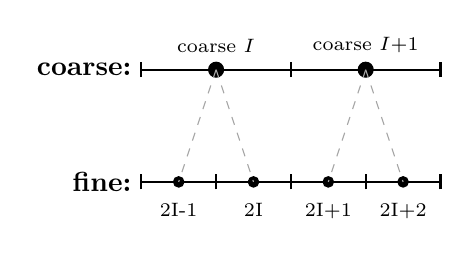
\begin{tikzpicture}[scale=0.95,>=stealth,line width=0.4pt]
  % Coarse cells (top row, large)
  \draw[thick] (0,1.5) -- (4,1.5);
  \foreach \x in {0,2,4} {\draw[thick] (\x,1.4) -- (\x,1.6);}
  \filldraw (1,1.5) circle (0.10);
  \filldraw (3,1.5) circle (0.10);
  \node[above] at (1,1.6) {\scriptsize coarse $I$};
  \node[above] at (3,1.6) {\scriptsize coarse $I{+}1$};
  \node[left] at (0,1.5) {\textbf{coarse:}};
  % Fine cells (bottom row, small)
  \draw[thick] (0,0) -- (4,0);
  \foreach \x in {0,1,2,3,4} {\draw[thick] (\x,-0.1) -- (\x,0.1);}
  \foreach \pos/\lab in {0.5/2I-1, 1.5/2I, 2.5/2I+1, 3.5/2I+2} {
    \filldraw (\pos,0) circle (0.07);
    \node[below] at (\pos,-0.15) {\scriptsize \lab};}
  \node[left] at (0,0) {\textbf{fine:}};
  % Mapping arrows
  \draw[dashed,gray!70] (1,1.5) -- (0.5,0);
  \draw[dashed,gray!70] (1,1.5) -- (1.5,0);
  \draw[dashed,gray!70] (3,1.5) -- (2.5,0);
  \draw[dashed,gray!70] (3,1.5) -- (3.5,0);
\end{tikzpicture}
\caption{Cell-centred coarsening on one axis.  The coarse cell at
index $I$ spans fine cells $2I{-}1$ and $2I$; the coarse-cell centre
lies midway between the two fine-cell centres (no coincident slot).
The cc transfer operators average / interpolate accordingly.}
\label{fig:cc-coarsening}
\end{figure}

\paragraph{Restriction.}
The cc restriction is the eight-point box average over the fine cells
whose centres lie inside the coarse cell:
\begin{equation}\label{eq:restrict-cc}
  (R_h^H d)_{IJK}
  \;=\; \tfrac{1}{8}\!\!
  \sum_{p,q,r\in\{-1,0\}}\!\! d_{2I+p,\,2J+q,\,2K+r}.
\end{equation}
All eight weights are $\frac{1}{8}$.  This is the natural restriction
when the coarse cell is the union of eight fine cells of equal
volume; it is exact on constants by inspection, second-order on
smooth fields by symmetry of the offsets about the coarse-cell
centre, and self-adjoint in the discrete $\ell^2$ inner product up
to a factor of~$8$.

\paragraph{Prolongation: standard cc trilinear weights.}
Let $u^H$ denote the coarse correction.  A fine cell at fine index
$i = 2I + p$ (with $p \in \{-1, 0\}$, encoding which half of the
coarse cell it sits in) has axial offset $\delta_x = -p$
(so $\delta_x = 1$ when $p = 0$, $\delta_x = -1$ when $p = -1$;
i.e.\ the fine cell is on the side $\delta_x$ of the coarse-cell
centre).  The standard tensor-product cc trilinear formula uses
per-axis weights $(\tfrac{3}{4}, \tfrac{1}{4})$ -- near coarse cell
gets $\tfrac{3}{4}$, far coarse cell on the same side gets
$\tfrac{1}{4}$:
\begin{equation}\label{eq:prolong-cc}
  (P_H^h u^H)_{2I+p_x,\,2J+p_y,\,2K+p_z}
  \;=\!\!\!
  \sum_{(s_x,s_y,s_z)\in\{0,\delta\}^3}\!\!
  w^{(x)}_{s_x}\,w^{(y)}_{s_y}\,w^{(z)}_{s_z}\;
  u^H_{I+s_x,\,J+s_y,\,K+s_z},
\end{equation}
where the per-axis weight is
$w^{(a)}_0 = \tfrac{3}{4}$ (near coarse cell) and
$w^{(a)}_{\delta_a} = \tfrac{1}{4}$ (far coarse cell, on the same
side as the fine cell).  Expanding the tensor product, the eight
weights are $\tfrac{27}{64}, \tfrac{9}{64}, \tfrac{9}{64},
\tfrac{9}{64}, \tfrac{3}{64}, \tfrac{3}{64}, \tfrac{3}{64},
\tfrac{1}{64}$ for the eight coarse cells (centre, three
face-adjacent, three edge-adjacent, one corner) -- the
direct analogue of the trilinear-bilinear weights for the cc
geometry.  Both the restriction \eqref{eq:restrict-cc} and the
prolongation \eqref{eq:prolong-cc} are second-order accurate; the
pair satisfies $P_H^h = 8\,(R_h^H)^T$ for the box-average inner
product, the cc analogue of the variational relation.

\paragraph{Prolongation: position-aware override at hybrid Dirichlet
vertices.}
The standard $(\tfrac{3}{4}, \tfrac{1}{4})$ split is correct when
both the near and far coarse cells are interior cells at distance
$h_c / 2$ and $3 h_c / 2$ from the fine cell centre, respectively.
At the fine cell adjacent to a hybrid Dirichlet vertex, the
\emph{far} coarse slot is the coarse Dirichlet vertex itself,
which sits at the boundary -- distance $h_c / 2$ \emph{plus} a
half-cell, not $3 h_c / 2$.  More precisely (see
\Cref{fig:axis-layouts}), the fine cell at axis index $i_p = 1$
lives at $a_a + h_p / 2$ relative to the lower-D boundary, while
the coarse vertex $u^H_{I=0}$ lives at $a_a$ and the coarse cell
centre $u^H_{I=1}$ lives at $a_a + h_c / 2 = a_a + h_p$.  Both
coarse slots are equidistant from the fine cell, so the
geometrically correct linear interpolation weights on that axis
are $(\tfrac{1}{2}, \tfrac{1}{2})$, not
$(\tfrac{3}{4}, \tfrac{1}{4})$.  The override fires whenever
\emph{this rank} owns the lower-D (or upper-D) boundary of the
hybrid axis \emph{and} the fine cell sits at the global index
$i_p = 1$ (or $i_p = N_a$, mirror form); on every other axis the
standard weights are used.  The eight prolongation weights for a
fine cell with $k$ axes in the override regime are still a tensor
product of the per-axis weights; e.g.\ at the global corner
$(i_p, j_p, k_p) = (1, 1, 1)$ of a D--N axis on every axis, each
of the eight contributing coarse slots gets weight $\tfrac{1}{8}$
(uniform).  The override preserves the second-order accuracy of
the unmodified cc-trilinear formula and, crucially, fixes a
hybrid-axis V-cycle convergence-rate degradation that the
unmodified formula caused.

\paragraph{Sign of the prolongation.}
Because the code's defect convention is $d = \Delta_h u - f$ rather
than $f - \Delta_h u$, the coarse correction $e_H$ solves
$A_H e_H = d_H$ (not $-d_H$), and the fine-grid update is
$u_h \leftarrow u_h - P_H^h e_H$.  Both \texttt{prolong\_var\_3d}
and \texttt{prolong\_var\_cc\_3d} therefore \emph{subtract} the
prolongated correction in place (\verb|pval[idx] -= update|).
Physical Dirichlet boundary slots are skipped by both prolongations
so the inhomogeneous Dirichlet data set by \texttt{apply\_bc\_3d}
is preserved across coarse-grid corrections; Neumann boundary slots
(ghost or vertex-on-hybrid) are not skipped, since on those faces
the boundary slot is an unknown and the correction is non-zero
there.

\subsection{Convergence rate of the model V-cycle}
For the constant-coefficient $d$-dimensional Laplacian discretised by
the standard $(2d{+}1)$-point stencil, with red-black Gauss--Seidel
smoothing, full-weighting restriction, and linear (trilinear in 3D)
interpolation, the asymptotic V-cycle convergence factor is bounded
above by approximately $0.1$--$0.2$ depending on the number of
pre/post-smoothing sweeps; the factor is independent of $h$
\cite[\S4]{trottenberg2001multigrid}.  Local Fourier analysis (LFA)
\cite[Appx.~A]{trottenberg2001multigrid} is the standard tool for
quantifying these rates.

% =============================================================================
\section{Implementation}\label{sec:implementation}
% =============================================================================

\subsection{Source-tree layout}
The code is layered.  From bottom to top:
\begin{description}[style=nextline,leftmargin=2em]
\item[\texttt{domain.\{c,h\}}] MPI Cartesian decomposition.  The
  function \texttt{automatic\_topology} chooses the process grid
  $(p_x,p_y,p_z)$ by greedy prime factorisation of the rank count;
  \texttt{setup\_3d\_domain} builds the Cartesian communicator and
  computes per-rank local extents and global offsets.
\item[\texttt{gf.\{c,h\}}] Grid-function containers.  \texttt{struct
  ngfs\_3d} holds the local sizes, origin, spacing, an array of
  variable slots (\texttt{vars[]}), pre-allocated face-buffers for
  ghost exchange, and parent/child pointers used to chain multigrid
  levels.
\item[\texttt{comm.\{c,h\}}] Ghost-zone synchronisation.  \texttt{sync\_var\_3d}
  packs faces, posts non-blocking sends/receives one axis at a time,
  and unpacks.
\item[\texttt{gauss\_seidel.\{c,h\}}] The smoother and the defect
  operator: \texttt{gauss\_seidel\_3d}, \texttt{calc\_defect\_3d},
  \texttt{apply\_bc\_3d}.
\item[\texttt{multigrid.\{c,h\}}] Hierarchy construction
  (\texttt{ngfs\_3d\_create\_hierarchy}), transfer operators
  (\texttt{inject\_var\_3d}, \texttt{restrict\_var\_3d},
  \texttt{prolong\_var\_3d} for D--D layouts;
  \texttt{restrict\_var\_cc\_3d}, \texttt{prolong\_var\_cc\_3d}
  for any layout with a Neumann face), and the V-cycle driver
  \texttt{vcycle\_3d}.  The dispatch helper \texttt{all\_axes\_cc}
  picks the cc pair on every level where at least one face is
  Neumann; pure-Dirichlet levels keep the vertex-centred pair.
\item[\texttt{io.\{c,h\}} and \texttt{HDF5BinaryWrite.\{c,h\}}]
  Per-rank HDF5 output.  Each rank writes
  \texttt{<dir>/rank\_<R>.h5}; metadata (dimensions, spacings,
  origins, per-face Neumann flags, has-neighbour flags) lives in a
  \texttt{/metadata} group, and each variable appears as a 3D dataset
  named \texttt{/<vname>}.  Multiple calls from the same rank append
  more datasets to the same file.  The post-processing helper
  \texttt{scripts/make\_xdmf.py} reads every \texttt{rank\_*.h5} in
  a run directory and writes a \texttt{multigrid.xmf} sidecar that
  ParaView/VisIt open directly as a single assembled grid.
\item[\texttt{parameter.\{cc,h\}} and \texttt{toml.hpp}] TOML parameter
  parsing.  \texttt{parameter.cc} is C++; the
  \texttt{parse\_parameter\_file} entry point is exposed as
  \texttt{extern "C"} so the C driver can link against it.
\item[\texttt{driver\_multigrid.c}] The top-level program: parameter
  parsing, grid set-up, RHS initialisation from
  \eqref{eq:manufactured}, the outer iteration loop, error reporting,
  and HDF5 output.
\end{description}
A small set of variable indices is fixed in \texttt{gauss\_seidel.h}:
\texttt{VAR\_SOL = 0} (the solution $u$),
\texttt{VAR\_RHS = 1} (the source $f$),
\texttt{VAR\_DEF = 2} (the defect $d = \Delta_h u - f$).

\subsection{MPI domain decomposition}\label{sec:domain}
Given $P$ MPI ranks and global grid dimensions $(N_x,N_y,N_z)$, the
function \texttt{automatic\_topology} computes a process grid
$(p_x,p_y,p_z)$ with $p_x p_y p_z = P$ via a greedy descent on the
prime factors of $P$, biasing each factor toward the longest current
axis to keep tile aspect ratios close to one.  \texttt{MPI\_Cart\_create}
produces the Cartesian communicator used everywhere downstream.  The
periodicity flags are zero in all directions, which matches the
Dirichlet boundary conditions; switching to periodic
boundaries requires changing this in \texttt{setup\_3d\_domain} (see
\Cref{sec:bc-periodic}).

A face is a \emph{physical boundary} of the global domain on this rank
when the corresponding neighbour rank does not exist
(\texttt{lower\_x\_rank == INVALID\_RANK} and analogous).  Boundary
conditions are applied only on those faces; faces shared with another
rank are handled by ghost exchange.

\begin{figure}[h]
\centering
\begin{minipage}{0.8\textwidth}
\centering
\begin{verbatim}
   ghost     interior cells (owned)        ghost
    | g | * | * | * | * | * | * | * | * | g |
    0   1                              N-2  N-1
   <----------- local_nx --------------->
\end{verbatim}
\end{minipage}
\caption{One-dimensional view of a per-rank tile.  The width-$g_s=1$
ghost layer on each side stores values owned by the neighbouring rank
(or the physical boundary).  The seven-point stencil at any interior
point reads at most one ghost cell on each axis.}\label{fig:ghost}
\end{figure}

\subsection{Smoother kernel: red-black Gauss--Seidel SOR}\label{sec:smoother-impl}
The function \texttt{gauss\_seidel\_3d} (\texttt{src/gauss\_seidel.c:86}) implements
\eqref{eq:sor} in red-black ordering with global parity
$c(i,j,k) = (g_i+g_j+g_k)\bmod 2$, where $g_i = \mathtt{local\_i0} + i$
is the global index of local point $i$.  Using the global parity --- not
the local parity --- guarantees that neighbouring ranks colour
shared-face neighbours consistently, regardless of where rank
boundaries fall.  Each iteration consists of a red sweep, a ghost
exchange and BC application, a black sweep, and another ghost+BC sync.

The stencil coefficients in the GS update are precomputed once per
level from $h_x,h_y,h_z$:
\begin{align*}
  D &= 2(h_x^2 h_y^2 + h_x^2 h_z^2 + h_y^2 h_z^2),\\
  c_x &= h_y^2 h_z^2 / D, \quad
  c_y = h_x^2 h_z^2 / D, \quad
  c_z = h_x^2 h_y^2 / D, \quad
  c_s = h_x^2 h_y^2 h_z^2 / D,
\end{align*}
so that
$\widetilde u_{ijk} = c_x(u_{i\pm 1,j,k}) + c_y(u_{i,j\pm 1,k}) + c_z(u_{i,j,k\pm 1})
- c_s f_{ijk}$.
The SOR update \eqref{eq:sor} is then $u_{ijk} \leftarrow (1-\omega)u_{ijk}
+ \omega \widetilde u_{ijk}$.

\subsection{Defect}\label{sec:defect}
\texttt{calc\_defect\_3d} (\texttt{src/gauss\_seidel.c:196}) evaluates
$d_{ijk} = (\Delta_h u)_{ijk} - f_{ijk}$ at every interior point,
zeros it on physical boundaries (so the defect is consistent with
Dirichlet BCs), reduces the local maximum modulus across the Cartesian
communicator with \texttt{MPI\_Allreduce(\dots, MPI\_MAX)}, and
synchronises the ghost layer of \texttt{VAR\_DEF} so that the
restriction stencil can read complete data on the next call.

\subsection{Hierarchy construction}\label{sec:hierarchy}
\texttt{ngfs\_3d\_create\_hierarchy} (\texttt{src/multigrid.c:228}) builds
the parent$\to$child linked list by repeatedly halving the cell counts
in each direction and doubling the spacings.  The same Cartesian
process grid is used at every level; coarsening reduces the per-rank
tile but never agglomerates ranks.  Coarsening stops when either:
\begin{enumerate}[label=(\roman*),leftmargin=*]
  \item the cell count in any direction is odd (so exact 2:1 coarsening
    is impossible), or
  \item the minimum number of interior cells per rank per direction,
    reduced across all ranks via \texttt{MPI\_Allreduce}, drops below
    the user-supplied \texttt{min\_cells} threshold.
\end{enumerate}
For maximum hierarchy depth the user should choose each $n_x,n_y,n_z$
of the form $2^p\cdot c$ with $c$ odd; the algorithm then reaches a
coarsest grid of $c+1$ points per axis (or stops earlier on the
\texttt{min\_cells} criterion).

\subsection{Transfer operators}\label{sec:prolongation}
The vertex-centred operators of \Cref{sec:transfer-dd} are implemented
in \texttt{inject\_var\_3d}, \texttt{restrict\_var\_3d},
\texttt{prolong\_var\_3d}; the cell-centred operators of
\Cref{sec:transfer-cc} are implemented in \texttt{restrict\_var\_cc\_3d}
and \texttt{prolong\_var\_cc\_3d}.  \texttt{vcycle\_3d} consults the
helper \texttt{all\_axes\_cc(level)} once per level and dispatches to
the cc pair when any axis has a Neumann face, the vertex-centred
pair otherwise.  Four implementation details are worth highlighting:
\begin{itemize}[leftmargin=*]
  \item \emph{Boundary handling in vertex-centred restriction.}
    The full-weighting stencil is applied only at interior coarse-grid
    points.  Coarse boundary points are first overwritten by injection
    from the fine-grid boundary, ensuring that homogeneous Dirichlet
    data on the fine grid carries through unchanged.  The cc
    restriction has no analogous boundary case: every owned coarse
    cell averages eight interior fine cells (no slot at the boundary).

  \item \emph{Sign of the prolongation.}  Because the code's defect
    convention is $d=\Delta_h u - f$ rather than $f - \Delta_h u$, the
    coarse correction $e_H$ is the solution of $A_H e_H = d_H$
    (\emph{not} $A_H e_H = -d_H$), and the fine-grid update is
    $u_h \leftarrow u_h - P_H^h e_H$.  Both \texttt{prolong\_var\_3d}
    and \texttt{prolong\_var\_cc\_3d} therefore subtract the
    prolongated correction in place
    (\verb|pval[idx] -= update|).  Physical Dirichlet boundary slots
    are skipped by both prolongations so inhomogeneous Dirichlet data
    set by \texttt{apply\_bc\_3d} is preserved across coarse-grid
    corrections; Neumann boundary slots (ghost or vertex-on-hybrid)
    are not skipped, since on those faces the boundary slot is an
    unknown and the correction is non-zero there.

  \item \emph{Position-aware weights at hybrid Dirichlet vertices.}
    \texttt{prolong\_var\_cc\_3d} computes six per-axis predicates
    (\texttt{x\_lower\_d\_v}, \texttt{x\_upper\_d\_v},
    \texttt{y\_lower\_d\_v}, etc.) at the top of the function -- each
    is true iff this rank owns the hybrid Dirichlet boundary on that
    side.  Inside the kernel, the per-axis interpolation weights flip
    from $(\tfrac{3}{4}, \tfrac{1}{4})$ to $(\tfrac{1}{2}, \tfrac{1}{2})$
    on any axis where the predicate is true \emph{and} the fine cell
    sits at global index $i_p = 1$ (lower D) or $i_p = N_a$ (upper D)
    on that axis.  The override fixes a hybrid-axis V-cycle
    convergence-rate degradation that the unmodified cc-trilinear
    formula caused (see \texttt{Plan.md} \S 6.1).

  \item \emph{Ghost requirement.}  Both trilinear stencils read up to
    one neighbouring coarse-grid slot in each direction, so the
    coarse correction's ghost layer must be valid before either
    prolongation is called.  In practice this is guaranteed because
    the smoother (the last operation on the coarse level before the
    recursion returns) leaves the ghost layer of \texttt{VAR\_SOL}
    synchronised.
\end{itemize}

\subsection{V-cycle}\label{sec:vcycle-impl}
\texttt{vcycle\_3d} (\texttt{src/multigrid.c:711}) implements
\Cref{alg:vcycle}.

\begin{lstlisting}[caption={V-cycle pseudocode (matches
\texttt{vcycle\_3d}).},label=alg:vcycle]
vcycle_3d(level, n_smooth, omega, tol, subcycles):
    gauss_seidel_3d(level, n_smooth, omega)         // pre-smoothing
    norm = calc_defect_3d(level)                    // VAR_DEF, ghosts synced
    if level.child != NULL and norm > tol:
        for it = 1 .. subcycles:
            zero level.child.VAR_SOL; apply_bc_3d
            inject_var_3d(level, VAR_DEF, child, VAR_RHS)
            restrict_var_3d(level, VAR_DEF, child, VAR_RHS)
            vcycle_3d(child, n_smooth, omega, tol, subcycles)
            sync_var_3d(level, VAR_SOL)             // ghosts of fine SOL
            gauss_seidel_3d(level, n_smooth, omega) // post-smooth (SOR)
            gauss_seidel_3d(level, n_smooth, 1.0)   // post-smooth (plain GS)
            norm = calc_defect_3d(level)
            if norm <= tol: break
    if level.parent != NULL:
        prolong_var_3d(level, VAR_SOL, level.parent, VAR_SOL)  // u -= e
    return norm
\end{lstlisting}

With \texttt{subcycles}~$=1$ this is the standard V-cycle.  With
\texttt{subcycles}~$>1$ the inner loop performs additional coarse-grid
visits per level until the defect tolerance is met or the budget is
exhausted, producing a behaviour intermediate between a V-cycle and a
W-cycle.

\paragraph{Why two post-smoothing passes?}\label{par:two-postsmooths}
The post-smooth runs first an SOR pass with the user's $\omega$ and
then a plain Gauss--Seidel pass ($\omega = 1$).  This is deliberate.

When $\omega > 1$ the SOR iteration accelerates convergence on the
slowly-varying error components but, depending on $\omega$, can have a
\emph{worse} smoothing factor on the highest-frequency modes than plain
Gauss--Seidel.  In the multigrid context the smoother does not need to
converge --- it needs to leave the high-frequency error small enough
that the coarse grid can resolve what remains.  For the seven-point
Laplacian, red-black Gauss--Seidel achieves a smoothing factor of $1/4$
\emph{independent of $h$} \cite[\S2.1]{trottenberg2001multigrid}; SOR
with $\omega \neq 1$ does not necessarily share that bound.

The two-pass post-smooth therefore decouples the two concerns: the SOR
sweep is responsible for accelerating the smooth-component error, and
the plain-GS sweep guarantees a robust smoothing factor on the
high-frequency component before the defect is recomputed and the cycle
either terminates or returns to the parent.  The cost is one extra
\texttt{n\_smooth} sweep per subcycle, which is small compared to the
$\bigO(N)$ work of the V-cycle as a whole and is the price of the code
tolerating any user-supplied $\omega \in (0,2)$.

\subsection{Driver loop}
The driver in \texttt{driver\_multigrid.c} reads the TOML file,
allocates the root grid with three variable slots, optionally builds
the hierarchy, initialises \texttt{VAR\_RHS} from
\eqref{eq:manufactured} and \texttt{VAR\_SOL}~$=0$, then iterates up to
\texttt{n\_iters} times.  Each iteration is either one V-cycle (if
\texttt{multigrid = true}) or one call to the smoother followed by a
defect computation; the loop terminates early if
$\norm{d}_{\Linf} < \texttt{tol}$.  After convergence the driver
computes $\norm{u_h - u_\star}_{\Linf}$ on the local interior, reduces
across ranks with \texttt{MPI\_MAX}, and prints the result.  Per-rank
HDF5 output is written by \texttt{output\_3d\_gf}, producing one
\texttt{rank\_<R>.h5} per process; the helper
\texttt{scripts/make\_xdmf.py} then writes a \texttt{multigrid.xmf}
sidecar that ParaView/VisIt open as a single assembled view.

% =============================================================================
\section{Building and running the code}\label{sec:build}
% =============================================================================

The build is CMake-driven and strictly out-of-tree: every object file,
library, executable, and test artefact lands under a user-chosen
\emph{build directory}, never in the \texttt{src/} tree.  The
top-level \texttt{CMakeLists.txt} lives in the project root and pulls
in \texttt{src/} via \verb|add_subdirectory|, so the typical commands
are run from the project root.

\subsection{Dependencies}\label{sec:build-deps}
\begin{description}[leftmargin=2em,style=nextline]
\item[MPI] Any standards-conforming implementation.  CMake locates the
  C and C++ wrappers via \verb|find_package(MPI REQUIRED COMPONENTS C CXX)|.
\item[HDF5] Required for per-rank output, located via
  \verb|find_package(HDF5 REQUIRED COMPONENTS C HL)|.  The \emph{serial}
  C library plus its High-Level helpers is sufficient -- each rank
  writes its own file, so a parallel-HDF5 build is not required.  On
  Fedora/RHEL install \texttt{hdf5-devel}; on Debian/Ubuntu install
  \texttt{libhdf5-dev}.
\item[Python 3 + h5py + numpy] Required by the test suite's verifiers
  and by \texttt{scripts/make\_xdmf.py}, which generates the XDMF
  sidecar that ParaView/VisIt use to open the per-rank output as a
  single assembled grid.
\end{description}

\subsection{Two build modes}\label{sec:build-modes}
The configuration is governed by two options.  The first selects what
to build, the second adjusts the compile flags:

\begin{description}[leftmargin=3em,style=nextline]
\item[\texttt{BUILD\_TESTING}] (default \texttt{OFF})
  When \texttt{OFF}, only the driver and its supporting libraries are
  built; CTest is not enabled.  Set it explicitly to \texttt{ON} for
  the configuration that the test suite expects.

\item[\texttt{MULTIGRID\_FAST\_MATH}] (auto-default)
  Adds \texttt{-ffast-math} to the compile flags.  The default is
  auto-selected from \texttt{BUILD\_TESTING}:
  \texttt{ON} when \texttt{BUILD\_TESTING=OFF} (full speed for
  production runs), and \texttt{OFF} when \texttt{BUILD\_TESTING=ON}
  (strict IEEE arithmetic so the convergence test in
  \Cref{sec:tuning} measures the true discretisation error rather
  than compiler reassociations).  Either default can be overridden
  on the \texttt{cmake} command line.
\end{description}

The configure-time status print
(\verb|-- BUILD_TESTING = ...|, \verb|-- MULTIGRID_FAST_MATH = ...|)
makes the resolved choice unmissable.

\subsection{Production workflow}\label{sec:build-prod}
\begin{lstlisting}[language=bash]
# from the project root
cmake -B build                                 # BUILD_TESTING=OFF, FAST_MATH=ON
cmake --build build -j
mpirun -np <N> build/src/driver_multigrid <params.toml>
\end{lstlisting}

\subsection{Test workflow}\label{sec:build-test}
\begin{lstlisting}[language=bash]
cmake -B build-test -DBUILD_TESTING=ON         # FAST_MATH=OFF auto
cmake --build build-test -j
ctest --test-dir build-test --output-on-failure
\end{lstlisting}

The CTest entries are labelled, so subsets can be run independently:
\verb|ctest -L operator| runs only the six operator-level unit tests
(domain decomposition, hierarchy construction, injection,
restriction, prolongation), and \verb|ctest -L end_to_end| runs only
the parser-hardening regression and the second-order-convergence
test described in \Cref{sec:tuning}.

\paragraph{Note.}
Running \verb|ctest --test-dir build| against a tree configured
without \verb|-DBUILD_TESTING=ON| reports
\texttt{No tests were found!} -- the test binaries and CTest
registrations are only generated when the option is set at configure
time.  Use a dedicated build directory (\texttt{build-test/} above)
or re-configure the existing tree with the option enabled.

\subsection{Cleaning}
\begin{lstlisting}[language=bash]
cmake --build build --target clean   # remove generated objects/binaries
rm -rf build                         # full reset, including test artefacts
\end{lstlisting}

% =============================================================================
\section{User-selectable parameters}\label{sec:parameters}
% =============================================================================

The driver takes a single command-line argument: the path to a TOML
parameter file.  An example (\texttt{multigrid.toml}) is shipped with
the code:
\begin{lstlisting}[language={},caption={Sample input file.}]
[grid]
nx_cells = 256
ny_cells = 256
nz_cells = 256

[solver]
multigrid = true
omega     = 1.5
n_smooth  = 100
n_iters   = 20
tol       = 1.0e-9
subcycles = 1
min_cells = 4
\end{lstlisting}

\subsection{Parameter reference}
\begin{table}[h]
\centering
\small
\begin{tabular}{@{}llp{0.62\linewidth}@{}}
\toprule
Section / key & Type & Meaning \\
\midrule
\verb|[grid].nx_cells| & positive int & Cells in $x$; grid points $= n_x{+}1$.  For deepest coarsening, prefer $n_x = 2^p\cdot c$ with $c$ odd. \\
\verb|[grid].ny_cells| & positive int & Cells in $y$. \\
\verb|[grid].nz_cells| & positive int & Cells in $z$. \\
\addlinespace
\verb|[solver].multigrid| & bool & \texttt{true}: V-cycle multigrid.  \texttt{false}: single-grid red-black Gauss--Seidel SOR. \\
\verb|[solver].omega|     & float $\in(0,2)$ & SOR relaxation parameter.  $\omega=1$ is plain Gauss--Seidel; $1<\omega<2$ is over-relaxation.  See \Cref{sec:tuning}. \\
\verb|[solver].n_smooth|  & positive int & Number of red-black GS iterations per smoothing call. \\
\verb|[solver].n_iters|   & positive int & Maximum number of outer iterations (V-cycles, or single-grid GS calls). \\
\verb|[solver].tol|       & non-negative float & Termination threshold on $\norm{d}_{\Linf}$. \\
\verb|[solver].subcycles| & positive int & (multigrid only) Maximum coarse-grid visits per level.  $1$ = V-cycle, $>1$ behaves like a partial W-cycle. \\
\verb|[solver].min_cells| & positive int & (multigrid only) Minimum interior cells per rank per direction.  Coarsening stops below this. \\
\bottomrule
\end{tabular}
\caption{Input parameters.}
\end{table}

\subsection{Practical tuning guidance}\label{sec:tuning}
\paragraph{$\omega$ (SOR parameter).}
For multigrid, the smoother only needs to damp high frequencies; a
common and robust choice is $\omega \in [1.0, 1.3]$ for red-black GS.
Higher values (closer to the single-grid optimum
\eqref{eq:omega-opt}) sometimes accelerate the smoother but can erode
the smoothing factor.  When running in single-grid mode, choose
$\omega$ near $\omega_{\mathrm{opt}}$; for $h \approx 1/256$ this gives
$\omega \approx 1.97$.  The shipped default $\omega=1.5$ is a
compromise that works for both modes on the example problem.

\paragraph{\texttt{n\_smooth}.}
Multigrid theory predicts that a small number of smoothing sweeps
($\nu_1 = \nu_2 = 1$ or $2$) is sufficient
\cite[\S4]{trottenberg2001multigrid}.  In practice, on a parallel
machine where ghost exchanges have non-trivial latency, larger
\texttt{n\_smooth} (between $4$ and the shipped $100$) can improve
\emph{strong-scaling} efficiency by amortising the communication cost
even though it does not change the asymptotic algorithmic complexity.
Tune for time-to-solution, not iteration count.

\paragraph{\texttt{n\_iters} and \texttt{tol}.}
Set \texttt{tol} to the target precision (typically a small multiple of
the discretisation error $\bigO(h^2)$) and \texttt{n\_iters} to a
generous upper bound; the loop exits early once the tolerance is met.

\paragraph{\texttt{subcycles}.}
Leave this at $1$ unless you observe that V-cycles plateau before the
defect drops to \texttt{tol}; in that case increasing it to $2$
behaves like a W-cycle on the affected levels and is the cheapest
remedy.

\paragraph{\texttt{min\_cells}.}
A small value (the default $4$) lets the hierarchy go as deep as
the grid allows.  On a very large rank count, $4$ may be too
aggressive: the coarsest level becomes communication-bound because each
rank holds only a handful of cells.  In that regime, $8$ or $16$ is
often a better choice.  At present the code does not implement
rank-agglomeration on coarse grids, which is the more sophisticated
remedy \cite[\S6.3]{trottenberg2001multigrid}.

\paragraph{\texttt{nx\_cells}, \texttt{ny\_cells}, \texttt{nz\_cells}.}
Powers of two maximise hierarchy depth.  Cell counts that are not
powers of two are accepted but bottom out at the first odd factor.

% =============================================================================
\section{Extending the code}\label{sec:extension}
% =============================================================================

For the most common extension --- a different right-hand side and
different boundary data on the same Poisson operator --- the code is
fully data-driven.  The smoother, V-cycle, transfer operators, and
boundary kernels do not need to be edited; the user supplies a small
record of callbacks (a \emph{problem preset}), the driver picks one up
by name from the TOML, and everything downstream is automatic.  This
is described in \Cref{sec:adding-preset}.

A second tier of extensions --- Robin and periodic boundary conditions,
variable coefficients, anisotropic operators --- still requires
modifying the kernels and is outlined in
\Cref{sec:bc-robin,sec:bc-periodic,sec:variable}.

\subsection{Adding a new problem: the preset workflow}\label{sec:adding-preset}

Every problem the driver can solve is encoded as a \texttt{problem\_t}
record in the registry table \texttt{g\_problems[]}, defined in
\texttt{src/problem\_registry.c}.  Adding a new problem is a one-file
edit: write a few pure C functions, append a record to the table,
rebuild.

\subsubsection{Anatomy of a preset}

The public interface is in \texttt{src/problem.h}:
\begin{lstlisting}
typedef double (*scalar_field_fn)(double x, double y, double z);
typedef double (*bc_fn_t)(double x, double y, double z, face_id_t face);

struct problem_t {
    const char        *name;     /* TOML key */
    struct bc_spec_t   bc;       /* per-face BC kinds + value callbacks */
    scalar_field_fn    rhs;      /* f(x,y,z); required */
    scalar_field_fn    u_exact;  /* optional (NULL if no closed form) */
    bool               singular; /* true => mean-zero projection */
};
\end{lstlisting}
The boundary specification \texttt{bc\_spec\_t} (in
\texttt{src/bc.h}) is six \texttt{bc\_face\_t} entries, one per face:
\begin{lstlisting}
struct bc_face_t {
    bc_kind_t kind;        /* BC_DIRICHLET or BC_NEUMANN */
    bool      homogeneous; /* true => value/flux is identically 0 */
    bc_fn_t   value;       /* ignored when homogeneous == true */
};
\end{lstlisting}
\texttt{problem\_registry.c} provides four convenience macros that
match the four common combinations:
\begin{lstlisting}
#define DIRICHLET_HOMOG_FACE          { BC_DIRICHLET, true,  NULL }
#define DIRICHLET_INHOMOG_FACE(cb)    { BC_DIRICHLET, false, (cb) }
#define NEUMANN_HOMOG_FACE            { BC_NEUMANN,   true,  NULL }
#define NEUMANN_INHOMOG_FACE(cb)      { BC_NEUMANN,   false, (cb) }
\end{lstlisting}
Face identifiers are \verb|FACE_LOWER_X|, \verb|FACE_UPPER_X|,
\verb|FACE_LOWER_Y|, \verb|FACE_UPPER_Y|, \verb|FACE_LOWER_Z|,
\verb|FACE_UPPER_Z|.

\subsubsection{Sign conventions}

The equation is $\Delta u = f$ on $\Omega = [0,1]^3$.  Each callback
takes the global $(x,y,z)$ coordinate of the boundary point and the
face identifier:
\begin{itemize}[leftmargin=*,nosep]
\item \emph{Dirichlet} callbacks return $u(\mathbf{x})$ at the face
  point --- the value the solver will pin on the boundary.
\item \emph{Neumann} callbacks return $\partial u/\partial n$, the
  outward-normal derivative.  Outward normals are
  $-\hat{x}, +\hat{x}, -\hat{y}, +\hat{y}, -\hat{z}, +\hat{z}$ at the
  six faces respectively, so on a lower face,
  $\partial u/\partial n = -\partial u/\partial x_i$ and the user is
  responsible for the sign flip.
\end{itemize}

\subsubsection{Singular flag}\label{sec:preset-singular}

Set \verb|singular = true| only when \emph{every} face is Neumann.
The driver then projects the discrete solution onto the mean-zero
subspace after each V-cycle to remove the constant null-space drift.
Pure Neumann also requires the discrete compatibility condition
$\int_\Omega f \, d\mathbf{x} = \int_{\partial\Omega} q \, dS$ to hold;
the implementation projects $f$ to mean-zero at startup (which handles
the homogeneous case) but does \emph{not} currently account for the
$\sum 2 q / h$ term that arises from the Neumann ghost-mirror
discretisation.  As documented in \texttt{Plan.md}, the
\texttt{manufactured\_neumann\_inhomog} preset (registered, but
deliberately excluded from the convergence-test suite) demonstrates
this limitation.  Mixed problems, where at least one face is
Dirichlet, are non-singular and have no analogous restriction --- set
\verb|singular = false|.

\subsubsection{Worked example}\label{sec:adding-preset-example}

To make the workflow concrete, take the manufactured solution
\begin{equation*}
  u^{\star}(x,y,z) \;=\; e^{x} \sin(\pi y) \cos(\pi z / 2),
\end{equation*}
which has $\nabla^{2} u^{\star} = (1 - 5\pi^{2}/4) \, u^{\star}$.
Inspecting the function on each face gives a problem with mixed BCs:
$x$ faces inhomogeneous Dirichlet, $y$ faces inhomogeneous Neumann,
lower-$z$ homogeneous Neumann (because $\sin(\pi z/2)$'s derivative
$\cos(\pi z/2)$ does not vanish at $z=0$, but
$\partial u^\star/\partial z = -(\pi/2) e^x \sin(\pi y) \sin(\pi z/2)$
does, since $\sin 0 = 0$), upper-$z$ inhomogeneous Neumann.

Step~1: open \texttt{src/problem\_registry.c} and add the callbacks
above the registry table:
\begin{lstlisting}
static double my_exact(double x, double y, double z)
{
    const double pi = 3.14159265358979323846;
    return exp(x) * sin(pi * y) * cos(pi * z / 2.0);
}
static double my_rhs(double x, double y, double z)
{
    const double pi = 3.14159265358979323846;
    return (1.0 - 5.0 * pi * pi / 4.0) * my_exact(x, y, z);
}
/* Dirichlet returns u_star at the face point. */
static double my_dirichlet(double x, double y, double z, face_id_t face)
{ (void)face; return my_exact(x, y, z); }
/* Neumann returns du/dn (outward) at the face point.
 * Lower-z is registered as NEUMANN_HOMOG_FACE so the lower-z case
 * never enters this switch. */
static double my_neumann(double x, double y, double z, face_id_t face)
{
    const double pi = 3.14159265358979323846;
    const double dudy =  pi       * exp(x) * cos(pi * y) * cos(pi * z / 2.0);
    const double dudz = -(pi/2.0) * exp(x) * sin(pi * y) * sin(pi * z / 2.0);
    switch (face) {
        case FACE_LOWER_Y: return -dudy;   /* outward normal -y */
        case FACE_UPPER_Y: return  dudy;
        case FACE_UPPER_Z: return  dudz;
        default:           return 0.0;     /* never reached */
    }
}
\end{lstlisting}

Step~2: append the preset to \texttt{g\_problems[]}, immediately before
the \verb|{ .name = NULL }| sentinel:
\begin{lstlisting}
{
    .name = "my_mixed_problem",
    .bc   = { .face = {
        [FACE_LOWER_X] = DIRICHLET_INHOMOG_FACE(my_dirichlet),
        [FACE_UPPER_X] = DIRICHLET_INHOMOG_FACE(my_dirichlet),
        [FACE_LOWER_Y] = NEUMANN_INHOMOG_FACE(my_neumann),
        [FACE_UPPER_Y] = NEUMANN_INHOMOG_FACE(my_neumann),
        [FACE_LOWER_Z] = NEUMANN_HOMOG_FACE,
        [FACE_UPPER_Z] = NEUMANN_INHOMOG_FACE(my_neumann),
    }},
    .rhs      = my_rhs,
    .u_exact  = my_exact,
    .singular = false,
},
\end{lstlisting}

Step~3: rebuild and run.  No driver edits, no kernel edits.
\begin{lstlisting}[language=bash]
cmake --build build -j
\end{lstlisting}

Step~4: write a TOML that selects the preset and run:
\begin{lstlisting}[language={}]
# my_run.toml
[grid]
nx_cells = 64
ny_cells = 64
nz_cells = 64

[solver]
multigrid = true
omega     = 1.0     # 1.0 is robust for Neumann/mixed; 1.5 is fine for pure Dirichlet
n_smooth  = 50
n_iters   = 60
tol       = 1.0e-12
subcycles = 1
min_cells = 4

[problem]
name = "my_mixed_problem"

[output]
dir = "out_run_001"  # optional; per-rank HDF5 (rank_<R>.h5) written here, mkdir -p'd by rank 0
\end{lstlisting}
\begin{lstlisting}[language=bash]
mpirun -np 4 build/src/driver_multigrid my_run.toml
\end{lstlisting}
The driver prints a per-iteration $\norm{d}_{\Linf}$ trace and, if a
\texttt{u\_exact} callback was supplied, the final
$\norm{u_{h} - u^{\star}}_{\Linf}$.

\subsubsection{Optional: register a CTest convergence check}

If the preset has an exact solution, the convergence-test harness can
verify that it converges at second order with no further code.  Add
the preset name to the \verb|CONVERGENCE_PRESETS| list in
\texttt{src/tests/CMakeLists.txt}:
\begin{lstlisting}[language={}]
set(CONVERGENCE_PRESETS
    manufactured_dirichlet_homog
    manufactured_dirichlet_inhomog
    manufactured_neumann_homog
    manufactured_mixed
    manufactured_mixed_inhomog
    my_mixed_problem        # <- new
)
\end{lstlisting}
Re-configure (\verb|cmake -B build-test -DBUILD_TESTING=ON|), build
the tests, and \verb|ctest --test-dir build-test -R convergence_my_mixed_problem|.
The harness runs the problem at $32^{3}$, $64^{3}$, $128^{3}$ on
both \texttt{np=1} and \texttt{np=8}, parses the printed
$\norm{u_{h} - u^{\star}}_{\Linf}$, and asserts a convergence rate in
$[1.8, 2.3]$ on the finest pair (see \Cref{sec:tuning} and
\texttt{tests/run\_test\_convergence.sh}).

\subsubsection{How the preset machinery hooks into the kernel}\label{sec:preset-internals}

Each \texttt{ngfs\_3d} carries a pointer \verb|struct bc_spec_t *bc|.
The driver stamps the preset's spec onto the root level once at
startup; \texttt{ngfs\_3d\_create\_child} (\texttt{multigrid.c}) calls
\texttt{bc\_spec\_homogenize} when constructing each coarse level,
which copies the parent's \texttt{kind} on every face but flips
\verb|homogeneous = true| and zeroes the callback pointer.  The
hard invariant of \Cref{sec:problem} --- coarse levels always carry
the homogeneous variant of the parent's BC kind, because the unknown
on a coarse level is the correction $e_{H}$ --- is therefore enforced
once at hierarchy-construction time and is invisible to the user
writing a preset.

The boundary kernels read \verb|gfs->bc| directly:
\begin{itemize}[leftmargin=*,nosep]
\item \texttt{apply\_bc\_3d} writes Dirichlet face values
  (\verb|cb(x,y,z,face)| or $0$ when homogeneous) and skips Neumann
  faces entirely (those are unknowns, updated by the smoother sweep).
\item \texttt{compute\_sweep\_bounds} (file-static in
  \texttt{gauss\_seidel.c}) widens the smoother and defect sweeps by
  one on every face this rank owns that is Neumann; at those
  boundary nodes, the inner stencil substitutes a ghost-mirror
  $u_{\text{ghost}} = u_{\text{interior}} + 2 h_n q$ for the
  off-domain neighbour (and reduces to $u_{\text{ghost}} =
  u_{\text{interior}}$ on homogeneous Neumann faces).
\item \texttt{prolong\_var\_3d} skips fine-grid physical boundary
  nodes only on Dirichlet faces; on Neumann faces the boundary node
  is an unknown and the correction is prolonged.
\end{itemize}

\subsection{Robin, $\alpha u + \beta \partial u/\partial n = r$}\label{sec:bc-robin}
Robin (or third-kind) boundary conditions interpolate between Dirichlet
($\beta=0$) and Neumann ($\alpha=0$) and are implemented by combining
the two ghost-row strategies above.  At the lower-$x$ face,
\begin{equation*}
  \alpha\, u_{0,j,k} + \beta\, \frac{u_{1,j,k} - u_{-1,j,k}}{2h_x}
  = r(\bx_{0,j,k}),
\end{equation*}
which solves for the ghost value
\begin{equation}\label{eq:robin-ghost}
  u_{-1,j,k} \;=\; u_{1,j,k} + \frac{2h_x}{\beta}\!\left[
    \alpha\, u_{0,j,k} - r(\bx_{0,j,k}) \right].
\end{equation}
Because $u_{-1,j,k}$ depends on $u_{0,j,k}$, the boundary equation is
typically eliminated by substituting \eqref{eq:robin-ghost} into the
seven-point stencil at $i=0$ and absorbing the $\alpha u_{0,j,k}$ term
into the diagonal.  Concretely, the modified equation for the
lower-$x$ boundary point becomes
\begin{equation}\label{eq:robin-eqn}
  \frac{2 u_{1,j,k} - 2 u_{0,j,k} - \tfrac{2h_x \alpha}{\beta} u_{0,j,k}
        + \tfrac{2h_x}{\beta} r}{h_x^2}
  + (\text{$y$ and $z$ second differences})
  = f_{0,j,k},
\end{equation}
i.e.\ a modified diagonal coefficient $-2/h_x^2 - 2\alpha/(h_x\beta)$ and
an additional contribution to the RHS of $-2 r / (h_x \beta)$.

In the code this is implemented by:
\begin{enumerate}[leftmargin=*,nosep]
\item Replacing \texttt{apply\_bc\_3d} on Robin faces with the
  ghost-update \eqref{eq:robin-ghost}.
\item Adding boundary-stencil branches to \texttt{gauss\_seidel\_3d}
  and \texttt{calc\_defect\_3d} that use \eqref{eq:robin-eqn} on
  Robin-boundary points.  A clean way to organise this is to
  precompute, on each rank that owns a Robin face, modified
  coefficient arrays (or a flat list of boundary-equation
  ``corrections'') so that the inner kernels remain branch-free.
\item Modifying \texttt{prolong\_var\_3d} to interpolate the
  correction at boundary points (Robin corrections are non-zero on
  the boundary).
\end{enumerate}
Note that on coarser levels the BC stays Robin with the \emph{same}
$\alpha$ and $\beta$ but the homogeneous data $r=0$ for the coarse-grid
correction --- the same homogenisation rule
\texttt{bc\_spec\_homogenize} already implements for the Dirichlet and
Neumann kinds (see \Cref{sec:preset-internals}).  In other words,
adding a Robin BC kind to the preset machinery requires both
(a)~extending \verb|bc_kind_t| with \verb|BC_ROBIN| (and a callback
that returns $\alpha$, $\beta$, $r$ at the face point), and
(b)~teaching the boundary kernels in \texttt{apply\_bc\_3d},
\texttt{gauss\_seidel\_3d}, \texttt{calc\_defect\_3d}, and
\texttt{prolong\_var\_3d} how to handle that case.  The first piece is
purely additive; the second is the bulk of the work.  Robin boundary
conditions are also discussed in \cite[\S2.3.2]{trottenberg2001multigrid}
in the multigrid context.

\subsection{Periodic boundary conditions}\label{sec:bc-periodic}
Periodicity is essentially free: it amounts to (i) flipping the
\texttt{periods} flags passed to \texttt{MPI\_Cart\_create} in
\texttt{setup\_3d\_domain} from $0$ to $1$ on the periodic axes (the
ghost exchange machinery in \texttt{sync\_var\_3d} then automatically
wraps), (ii) skipping the corresponding writes in \texttt{apply\_bc\_3d},
and (iii) removing the boundary \verb|continue| guards in
\texttt{prolong\_var\_3d} on the periodic axes.  Pure-periodic problems
share the singular-operator issue with pure-Neumann and require the
same compatibility-and-projection treatment.

\subsection{Variable-coefficient or anisotropic operators}\label{sec:variable}
For $\nabla\!\cdot\!(a(\bx)\nabla u) = f$ or strongly anisotropic
operators ($h_x \ll h_y$), the geometric multigrid components in this
code may degrade.  Practical extensions include:
\begin{itemize}[leftmargin=*,nosep]
\item rewriting the inner kernels of \texttt{gauss\_seidel\_3d} and
  \texttt{calc\_defect\_3d} to use the new stencil (the colouring,
  ghost exchange, and BC handling carry over unchanged);
\item using a \emph{Galerkin} coarse operator $A_H = R_h^H A_h
  P_H^h$ instead of re-discretising on each level
  \cite[\S5.4]{trottenberg2001multigrid}, which requires storing the
  operator on every level rather than just the spacings;
\item considering algebraic multigrid (AMG) for problems where the
  geometric coarsening hierarchy is poorly matched to the operator
  \cite[Appx.~A]{trottenberg2001multigrid}.
\end{itemize}

% =============================================================================
\section*{Acknowledgements and further reading}
% =============================================================================
The presentation here closely follows
\cite{briggs2000multigrid,trottenberg2001multigrid}; the parallel
considerations are standard MPI material as in
\cite{gropp2014using}; the finite-difference background is
\cite{leveque2007finite}.  For deeper analytical foundations of
multigrid the reader is referred to \cite{hackbusch1985multi}.

\begin{thebibliography}{99}

\bibitem{brandt1977multilevel}
A.~Brandt.
\newblock Multi-Level Adaptive Solutions to Boundary-Value Problems.
\newblock \emph{Mathematics of Computation}, 31(138):333--390, 1977.

\bibitem{briggs2000multigrid}
W.~L. Briggs, V.~E. Henson, and S.~F. McCormick.
\newblock \emph{A Multigrid Tutorial}.
\newblock SIAM, Philadelphia, 2nd edition, 2000.
\newblock ISBN 978-0-89871-462-3.

\bibitem{evans2010pde}
L.~C. Evans.
\newblock \emph{Partial Differential Equations}.
\newblock American Mathematical Society, 2nd edition, 2010.

\bibitem{fedorenko1964relaxation}
R.~P. Fedorenko.
\newblock The speed of convergence of one iterative process.
\newblock \emph{USSR Computational Mathematics and Mathematical Physics},
  4(3):227--235, 1964.

\bibitem{golub2013matrix}
G.~H. Golub and C.~F. Van~Loan.
\newblock \emph{Matrix Computations}.
\newblock Johns Hopkins University Press, 4th edition, 2013.

\bibitem{gropp2014using}
W.~Gropp, E.~Lusk, and A.~Skjellum.
\newblock \emph{Using MPI: Portable Parallel Programming with the
  Message-Passing Interface}.
\newblock MIT Press, 3rd edition, 2014.

\bibitem{hackbusch1985multi}
W.~Hackbusch.
\newblock \emph{Multi-Grid Methods and Applications}.
\newblock Springer-Verlag, Berlin, 1985.

\bibitem{leveque2007finite}
R.~J. LeVeque.
\newblock \emph{Finite Difference Methods for Ordinary and Partial
  Differential Equations: Steady-State and Time-Dependent Problems}.
\newblock SIAM, Philadelphia, 2007.

\bibitem{saad2003iterative}
Y.~Saad.
\newblock \emph{Iterative Methods for Sparse Linear Systems}.
\newblock SIAM, Philadelphia, 2nd edition, 2003.

\bibitem{trottenberg2001multigrid}
U.~Trottenberg, C.~W. Oosterlee, and A.~Sch{\"u}ller.
\newblock \emph{Multigrid}.
\newblock Academic Press, San Diego, 2001.

\bibitem{varga2009matrix}
R.~S. Varga.
\newblock \emph{Matrix Iterative Analysis}.
\newblock Springer, second revised and expanded edition, 2000.

\bibitem{young1971iterative}
D.~M. Young.
\newblock \emph{Iterative Solution of Large Linear Systems}.
\newblock Academic Press, New York, 1971.

\end{thebibliography}

\end{document}
